%---------------------------------------------------------------------
%
%                          Cap�tulo 1
%
%---------------------------------------------------------------------


\chapter{Proteopathogen, a protein database for studying \textit{Candida albicans} - host interaction}
\cabeceraEspecial{Proteopathogen}


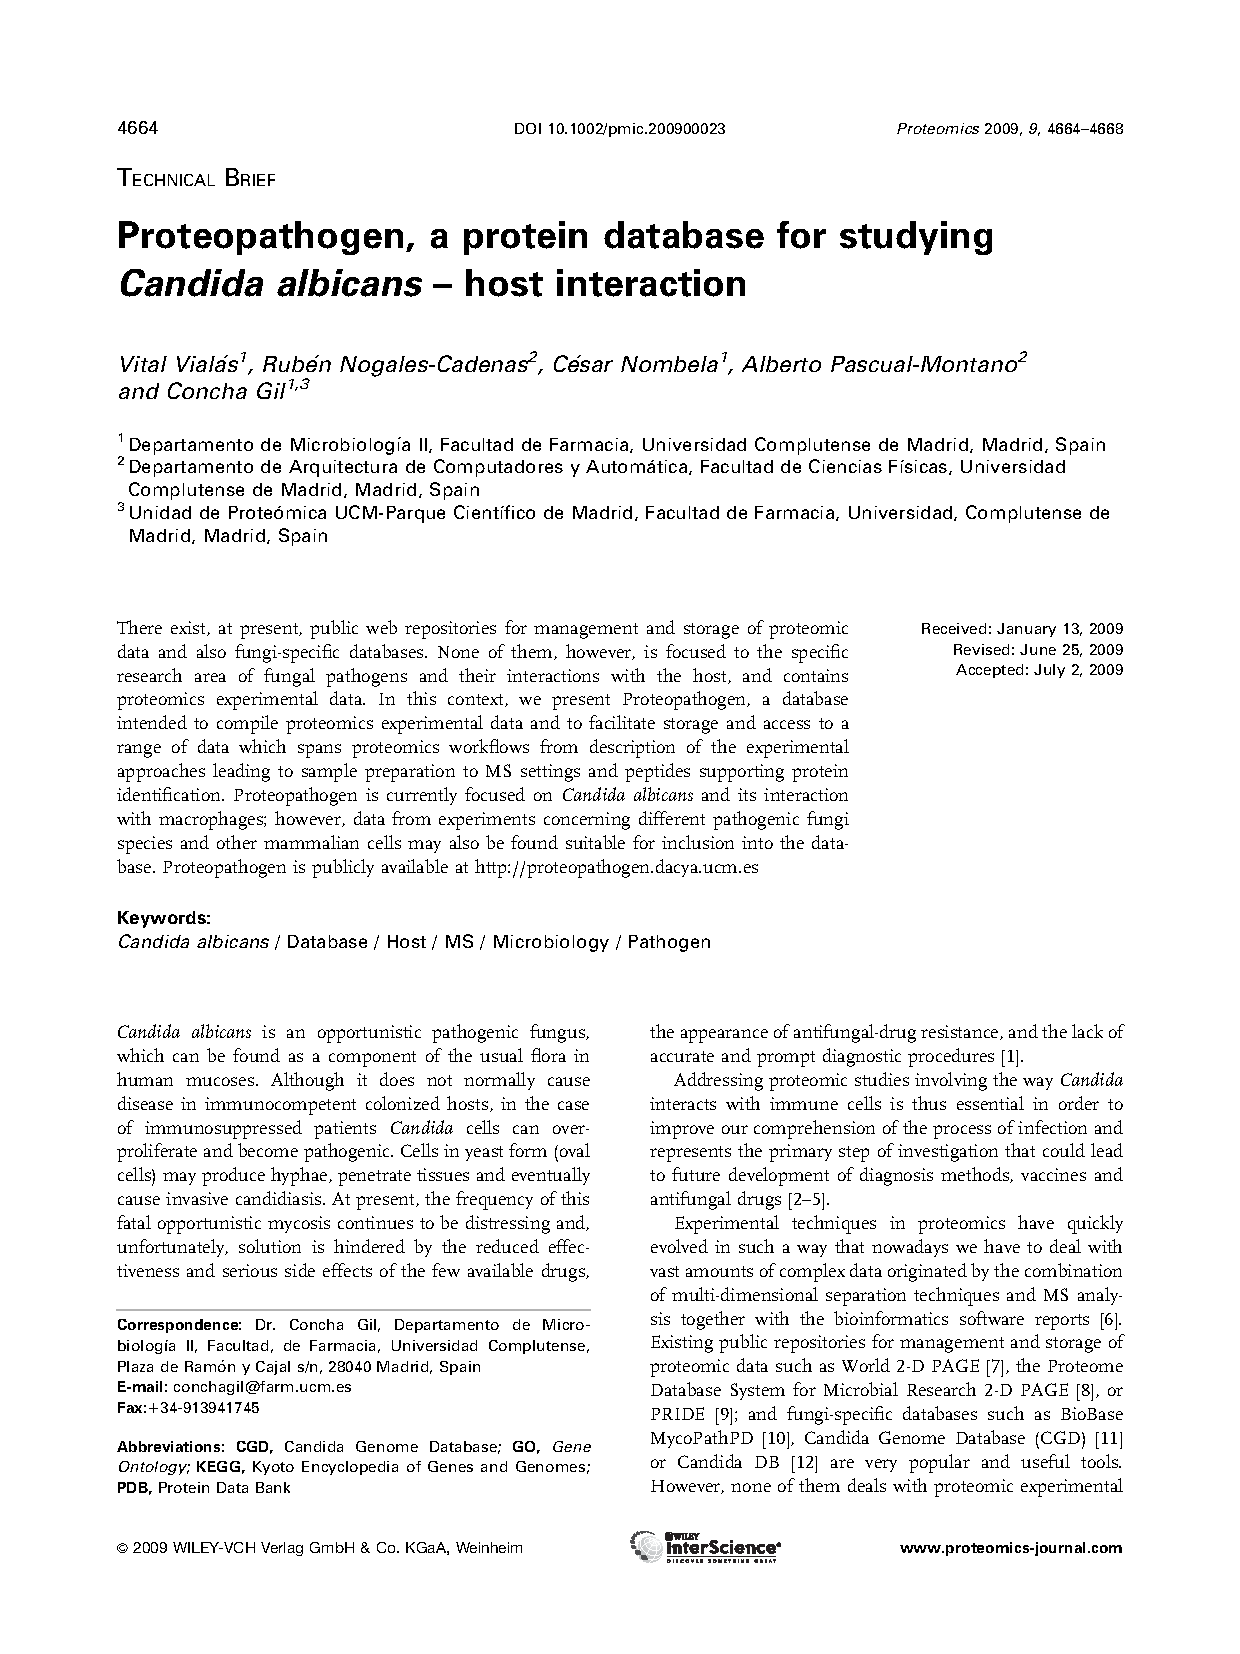
\includepdf[pages=-,scale=.85,pagecommand={}]{Capitulos/Vialas_2009_Proteopathogen_Proteomics.pdf}


%\begin{FraseCelebre}
%\begin{Frase}
%...
%\end{Frase}
%\begin{Fuente}
%...
%\end{Fuente}
%\end{FraseCelebre}

%\begin{resumen}
%...
%\end{resumen}


%-------------------------------------------------------------------
%\section{}


%-------------------------------------------------------------------
%\label{}

...

%-------------------------------------------------------------------
%\section*{\NotasBibliograficas}
%-------------------------------------------------------------------
%\TocNotasBibliograficas

%Citamos algo para que aparezca en la bibliograf�a\ldots
%\citep{ldesc2e}

%\medskip

%Y tambi�n ponemos el acr�nimo \ac{CVS} para que no cruja.

%Ten en cuenta que si no quieres acr�nimos (o no quieres que te falle la compilaci�n en ``release'' mientras no tengas ninguno) basta con que no definas la constante \verb+\acronimosEnRelease+ (en \texttt{config.tex}).


%-------------------------------------------------------------------
%\section*{\ProximoCapitulo}
%-------------------------------------------------------------------
%\TocProximoCapitulo

...

% Variable local para emacs, para  que encuentre el fichero maestro de
% compilaci�n y funcionen mejor algunas teclas r�pidas de AucTeX
%%%
%%% Local Variables:
%%% mode: latex
%%% TeX-master: "../Tesis.tex"
%%% End:
